\documentclass[aspectratio=169]{beamer}
\usepackage[T1]{fontenc}
\usepackage{lmodern}
\usepackage{tikz}
\usepackage{xcolor}
\usetikzlibrary{positioning, arrows.meta, shapes.geometric, shapes.misc, fit, calc, backgrounds}
\usetheme{metropolis}
\usefonttheme{professionalfonts}
\setbeamertemplate{footline}{}
\setbeamertemplate{navigation symbols}{}
\setbeamerfont{frametitle}{size=\large}

\definecolor{BlueA}{HTML}{174A7E}
\definecolor{BlueB}{HTML}{E4F0FB}
\definecolor{OrangeA}{HTML}{B46A1E}
\definecolor{OrangeB}{HTML}{FAEBD7}
\definecolor{GrayA}{HTML}{59636E}
\definecolor{GrayB}{HTML}{EEF2F5}
\definecolor{PurpleA}{HTML}{5B4B8A}
\definecolor{PurpleB}{HTML}{EEEAF8}
\definecolor{GreenA}{HTML}{2D7D46}
\definecolor{GreenB}{HTML}{E4F5E7}
\definecolor{RedA}{HTML}{A93433}
\definecolor{Ghost}{HTML}{AEB7C2}

\tikzset{
  box/.style={draw, rounded corners=3pt, align=center, font=\small,
              minimum height=1.15cm, minimum width=2.7cm, inner sep=5pt,
              very thick},
  env/.style={fill=OrangeB, draw=OrangeA},
  orch/.style={fill=BlueB, draw=BlueA},
  sub/.style={fill=PurpleB, draw=PurpleA},
  add/.style={fill=GreenB, draw=GreenA, very thick},
  ghost/.style={draw=Ghost, fill=white, text=GrayA, semithick},
  mem/.style={cylinder, shape border rotate=90, aspect=0.22, draw=GrayA,
              fill=GrayB, align=center, font=\scriptsize, minimum width=2.6cm,
              minimum height=1.4cm},
  arr/.style={-{Latex[length=2mm]}, thick},
  arr2/.style={{Latex[length=2mm]}-{Latex[length=2mm]}, thick},
  garr/.style={-{Latex[length=2mm]}, semithick, draw=Ghost},
  lbl/.style={font=\scriptsize, text=GrayA, fill=white, inner sep=1.5pt},
  glbl/.style={font=\scriptsize, text=GrayA},
}
\newcommand{\code}[1]{\texttt{\footnotesize #1}}

\begin{document}

% ===== PAGE 1: original runtime loop =====
\begin{frame}{Original Symbolica: one orchestrator-rooted LLM tree}
\centering
{\scriptsize\color{GrayA} infra (unchanged): LLM calls $\to$ agentica-server\,:2345
$\to$ TRAPI proxy\,:9091 (Bearer$\to$AAD) $\to$ agl-dev\,/\,TRAPI gpt-5.5}\\[0.7em]
\resizebox{!}{0.49\textheight}{%
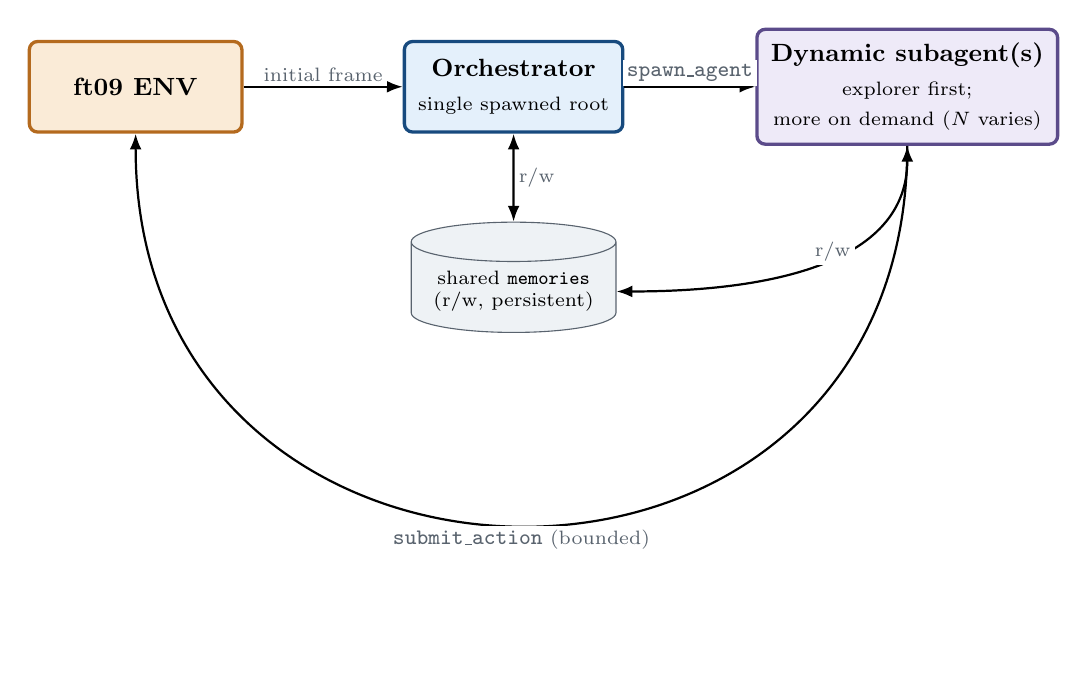
\begin{tikzpicture}
  \node[box, env]  (env)  at (0,0)    {\textbf{ft09 ENV}};
  \node[box, orch] (orch) at (4.8,0)  {\textbf{Orchestrator}\\[1pt]\scriptsize single spawned root};
  \node[box, sub]  (sub)  at (9.8,0)  {\textbf{Dynamic subagent(s)}\\[1pt]\scriptsize explorer first;\\\scriptsize more on demand ($N$ varies)};
  \node[mem, minimum height=1.05cm] (mem) at (4.8,-2.6){shared \texttt{memories}\\(r/w, persistent)};

  \draw[arr] (env)  -- node[lbl,above]{initial frame} (orch);
  \draw[arr] (orch) -- node[lbl,above]{\code{spawn\_agent}} (sub);
  \draw[arr2] (orch) -- node[lbl,right]{r/w} (mem);
  \draw[arr2] (sub.south) to[out=-90,in=0] node[lbl,above right]{r/w} (mem.east);
  \draw[arr] (sub.south) to[out=-90,in=-90,looseness=1.7]
       node[lbl,below]{\code{submit\_action} (bounded)} (env.south);
\end{tikzpicture}}

\vspace{0.5em}
{\footnotesize No skills: byte-identical original Symbolica --- one orchestrator
dynamically spawns subagents sharing \texttt{memories}, acting via bounded
\code{submit\_action}.}
\end{frame}

% ===== PAGE 2: trace2skill additive overlay =====
\begin{frame}{Trace2Skill: same loop $+$ one additive skill directory}
\centering
\resizebox{!}{0.50\textheight}{%
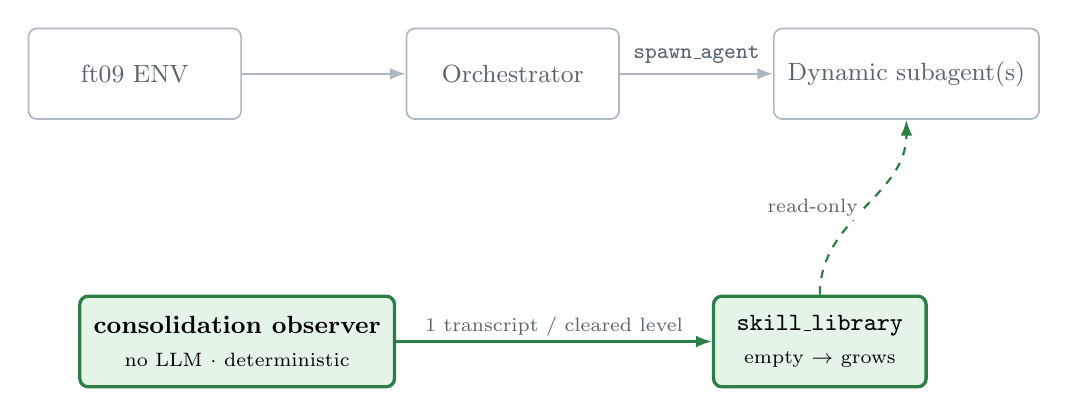
\begin{tikzpicture}
  % ---- ghosted page-1 base (faint, the unchanged runtime) ----
  \node[box, ghost] (env)  at (0,0)   {ft09 ENV};
  \node[box, ghost] (orch) at (4.8,0) {Orchestrator};
  \node[box, ghost] (sub)  at (9.8,0) {Dynamic subagent(s)};
  \draw[garr] (env)  -- (orch);
  \draw[garr] (orch) -- node[glbl,above]{\code{spawn\_agent}} (sub);

  % ---- the ONLY additions (highlighted, well separated below) ----
  \node[box, add] (cons) at (1.3,-3.4)
       {\textbf{consolidation observer}\\[1pt]\scriptsize no LLM $\cdot$ deterministic};
  \node[box, add] (lib)  at (8.7,-3.4)
       {\textbf{\texttt{skill\_library}}\\[1pt]\scriptsize empty $\to$ grows};

  \draw[arr, draw=GreenA] (cons) -- node[lbl,above]
       {1 transcript / cleared level} (lib);
  \draw[arr, draw=GreenA, dashed] (lib) to[out=90,in=-90]
       node[lbl,left]{read-only} (sub.south);
\end{tikzpicture}}

\vspace{0.5em}
{\footnotesize Trace2Skill adds only a fresh per-run \texttt{skill\_library}: a
deterministic observer records each cleared level's \textbf{verbatim action
transcript}. Trace-verified: this text re-enters the LLM \code{body.input}
after consolidation (87/145); causal reliance \emph{not} tested.}
\end{frame}

% ===== PAGE 3: result =====
\begin{frame}{Observed: trace2skill $\geq$ none on level (5/5, directional)}
\centering
\vspace{0.3em}
\begin{columns}[c]
\column{0.56\textwidth}
\footnotesize
\resizebox{\linewidth}{!}{%
\begin{tabular}{@{}l l@{}}
\hline
same-seed \code{trace2skill} $\geq$ \code{none} on level & \textbf{5/5} \\
\code{s47} \code{trace2skill} & \textcolor{GreenA}{\textbf{clean L6 WIN}} \\
\code{s47} \code{none} & stalled \textbf{L4} \\
skill text in LLM \code{body.input} & \textcolor{GreenA}{\textbf{trace-verified}} \\
\quad (post-consolidation) & 87/145 \\
causal reliance on skill & \textbf{not tested} \\
evidence strength & 8/9 M3-censored \\
claim boundary & \textbf{not clean-rev4} \\
\hline
\end{tabular}}
\column{0.40\textwidth}
\resizebox{\linewidth}{!}{%
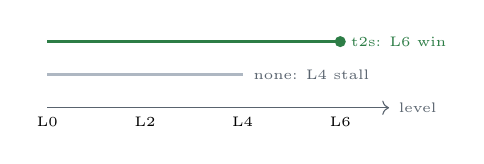
\begin{tikzpicture}[x=0.62cm,y=0.42cm]
  \draw[->,GrayA] (0,0) -- (7,0) node[right,font=\tiny]{level};
  \foreach \l in {0,2,4,6} \node[font=\tiny,below] at (\l,0) {L\l};
  \draw[Ghost, very thick] (0,1.0) -- (4,1.0)
        node[right,font=\tiny,text=GrayA]{none: L4 stall};
  \draw[GreenA, very thick] (0,2.0) -- (6,2.0)
        node[right,font=\tiny,text=GreenA]{t2s: L6 win};
  \fill[GreenA] (6,2.0) circle (2pt);
\end{tikzpicture}}
\end{columns}

\vspace{0.8em}
{\footnotesize \code{s47}: an empty directory grew to \textbf{5} verbatim action
transcripts that re-enter the LLM input; \code{trace2skill} reached \textbf{L6}
where \code{none} stalled at \textbf{L4} --- directional, causal use untested.\par}
\end{frame}

\end{document}
